\documentclass{ntuabeamer}

\usepackage[utf8]{inputenc}
\usepackage{amsmath}
\usepackage{amssymb}
\usepackage{booktabs}
\usepackage{graphicx}
\usepackage{tikz}
\usepackage{pgfplots}
\pgfplotsset{compat=1.18}
\usetikzlibrary{arrows.meta,positioning}

\title{Generalization and Regularization}
\author{}
\date{}
\graphicspath{{assets/}{assets/generated/}{assets/source/}}

\definecolor{courseblue}{HTML}{3F7CAC}
\definecolor{courseorange}{HTML}{D97706}
\definecolor{coursegreen}{HTML}{27864A}
\definecolor{coursepurple}{HTML}{7656A3}
\definecolor{coursered}{HTML}{B5473C}
\definecolor{coursegray}{HTML}{667085}
\definecolor{courselightblue}{HTML}{DCE9F5}
\definecolor{courselightorange}{HTML}{F9E4C8}

\begin{document}

\begin{frame}[plain]
  \makepresentationtitle
\end{frame}

\begin{frame}{Training Error Estimates a Population Quantity}
  For a future pair $(X,Y)\sim p_{\mathrm{data}}$, the target is
  \[
    R(\boldsymbol\theta)
    =\mathbb E[\ell(f_{\boldsymbol\theta}(X),Y)].
  \]
  The training sample provides
  \[
    L(\boldsymbol\theta)
    =\frac1n\sum_{i=1}^n\ell(f_{\boldsymbol\theta}(\mathbf x_i),y_i).
  \]
  Optimization reduces $L$. Generalization asks whether the selected model also has small $R$.
\end{frame}

\begin{frame}{Capacity Can Help Training and Hurt Validation}
  \centering
  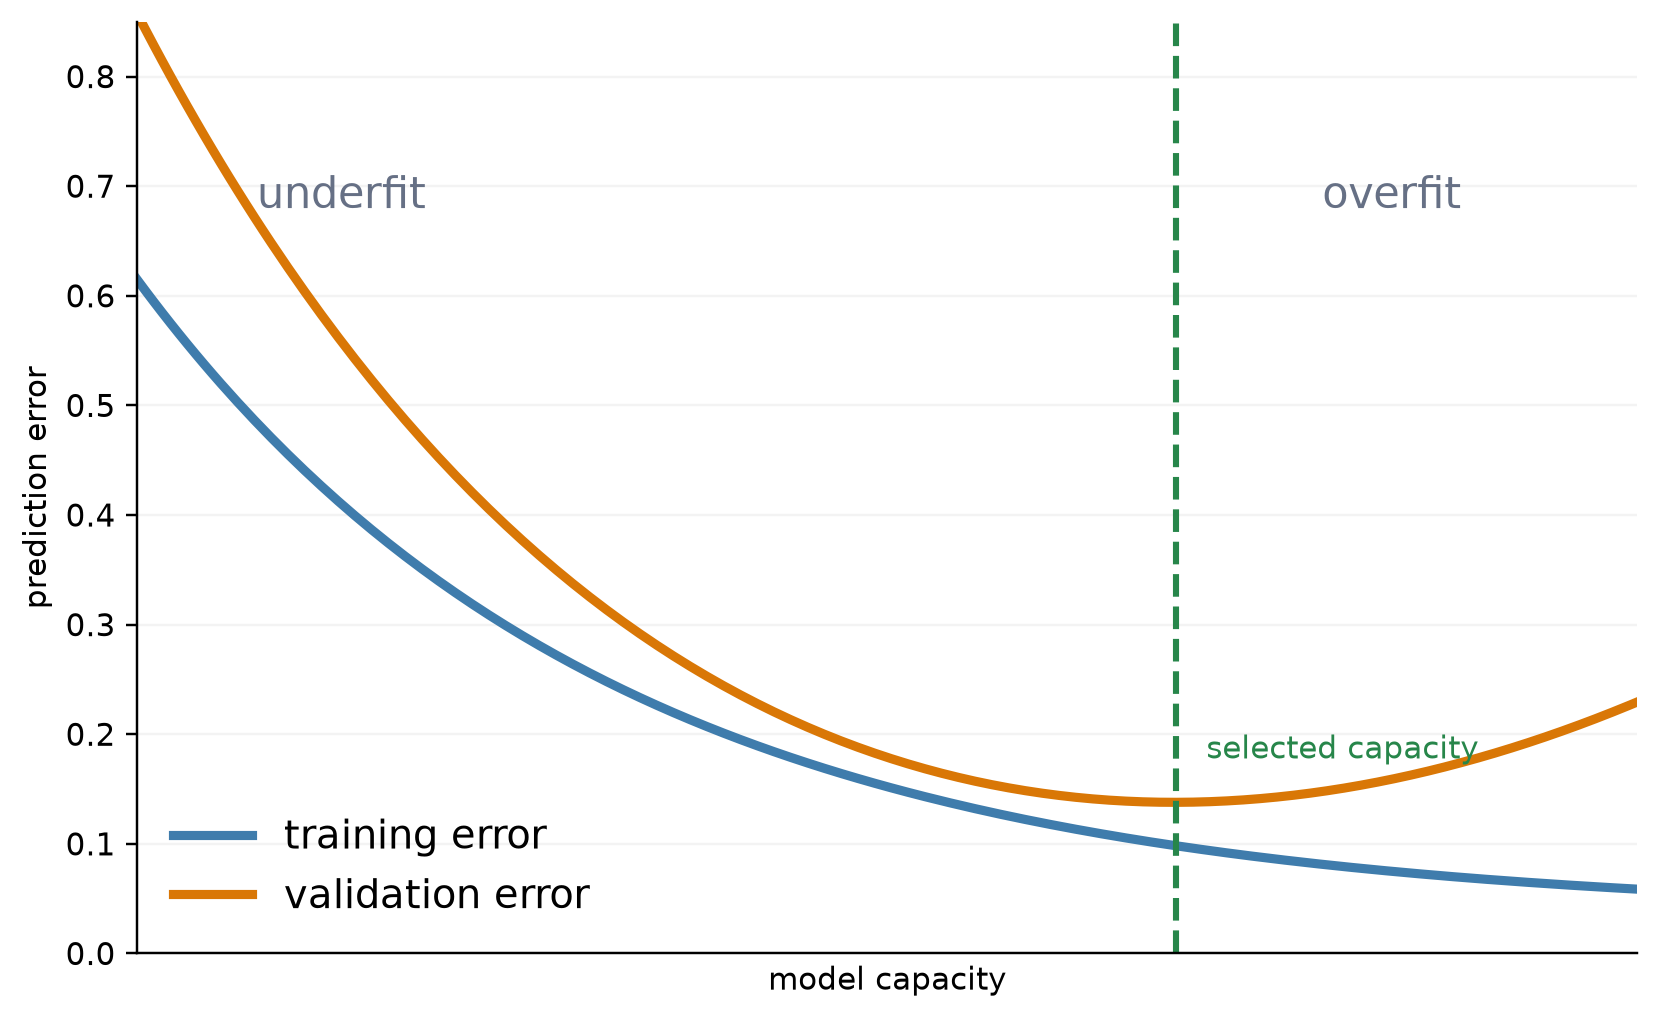
\includegraphics[width=0.95\linewidth,height=0.78\textheight,keepaspectratio]{learning-curves.png}
\end{frame}

\begin{frame}{Underfitting and Overfitting Are Different Failures}
  \begin{itemize}
    \item \textbf{Underfitting:} the model class or training procedure cannot capture useful structure.
    \item \textbf{Overfitting:} the fitted model responds too strongly to accidental details of the training sample.
  \end{itemize}
  \[
    \begin{aligned}
      L_{\mathrm{train}}\text{ high},\ L_{\mathrm{val}}\text{ high}
        &\ \Longrightarrow\ \text{underfitting},\\
      L_{\mathrm{train}}\text{ low},\ L_{\mathrm{val}}\text{ high}
        &\ \Longrightarrow\ \text{overfitting}.
    \end{aligned}
  \]
  More optimization can help the first case and worsen the second. Diagnose before choosing a remedy.
\end{frame}

\begin{frame}{Bias Is Systematic Error Across Possible Datasets}
  Let $\widehat f_D$ be the estimator trained on random dataset $D$. At input $x$,
  \[
    \operatorname{Bias}[\widehat f(x)]
    =\mathbb E_D[\widehat f_D(x)]-f(x).
  \]
  High bias means the \emph{average fitted prediction} is wrong.
  It is not the intercept parameter called ``bias'' in a neural layer.
\end{frame}

\begin{frame}{Variance Is Sensitivity to the Observed Dataset}
  \[
    \operatorname{Var}[\widehat f(x)]
    =\mathbb E_D\!\left[
      \left(\widehat f_D(x)-\mathbb E_D[\widehat f_D(x)]\right)^2
    \right].
  \]
  High variance means retraining on another sample from the same population changes the prediction strongly.
  This is estimator variance, not observation noise.
\end{frame}

\begin{frame}{Repeated Datasets Reveal Bias and Variance}
  \centering
  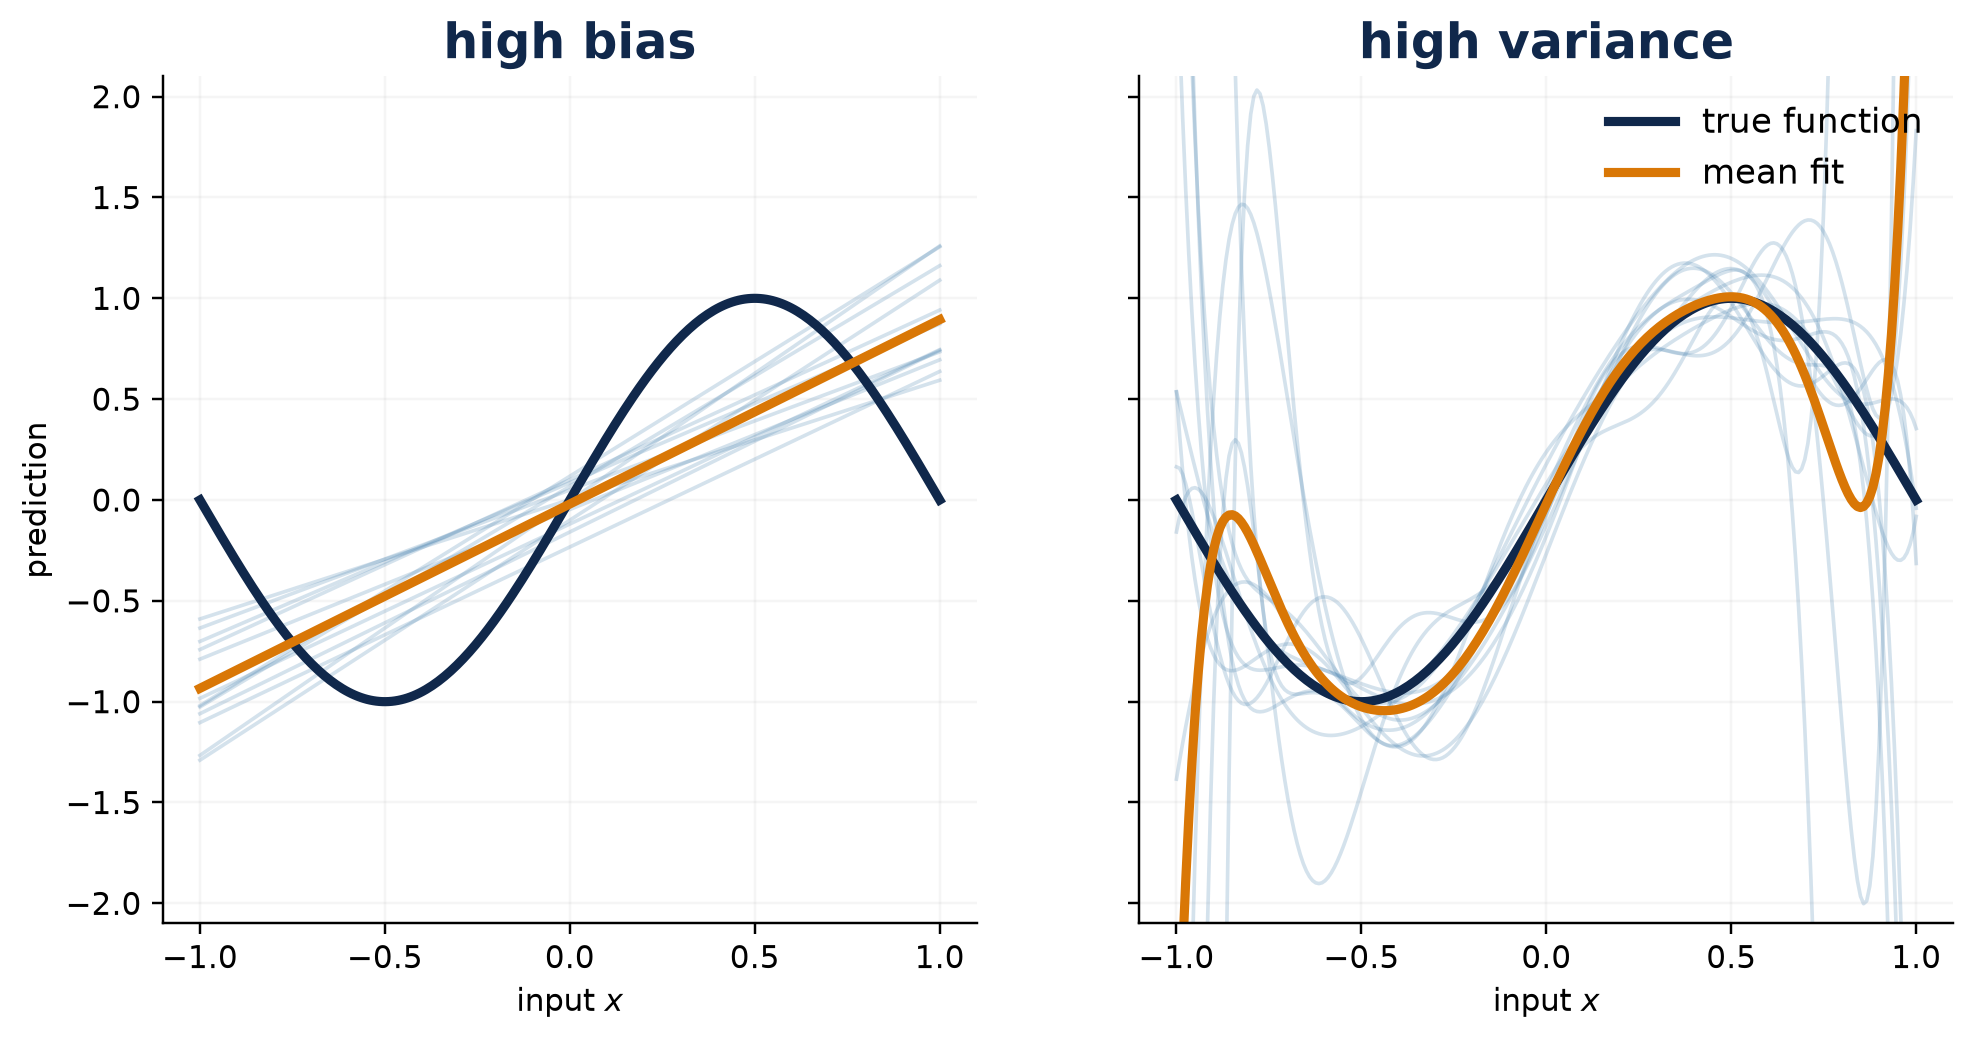
\includegraphics[width=0.98\linewidth,height=0.78\textheight,keepaspectratio]{bias-variance.png}
\end{frame}

\begin{frame}{Noise Is Error No Estimator Can Remove}
  Assume
  \[
    Y=f(X)+\varepsilon,
    \qquad \mathbb E[\varepsilon\mid X]=0,
    \qquad \operatorname{Var}(\varepsilon\mid X=x)=\sigma^2(x).
  \]
  Even the true regression function $f(x)=\mathbb E[Y\mid X=x]$ has conditional squared error $\sigma^2(x)$.
  Better data can reduce uncertainty about $f$; it cannot remove randomness in $Y\mid X$.
\end{frame}

\begin{frame}{Squared Error Decomposes into Three Terms}
  At a fixed $x$, with training data independent of the new observation,
  \[
    \boxed{
    \mathbb E_{D,Y\mid x}[(Y-\widehat f_D(x))^2]
    =\sigma^2(x)
    +\operatorname{Bias}[\widehat f(x)]^2
    +\operatorname{Var}[\widehat f(x)]}.
  \]
  Noise belongs to the data-generating process. Bias and variance belong to the learning procedure and its data.
\end{frame}

\begin{frame}{The Cross Terms Vanish by Centering}
  Add and subtract $f(x)$ and $\bar f(x)=\mathbb E_D[\widehat f_D(x)]$:
  \[
    Y-\widehat f_D
    =\underbrace{Y-f}_{\varepsilon}
     +\underbrace{f-\bar f}_{-\mathrm{Bias}}
     +\underbrace{\bar f-\widehat f_D}_{\text{centered estimator}}.
  \]
  Squaring and taking expectations removes cross terms because
  \[
    \mathbb E[\varepsilon\mid x]=0,
    \qquad
    \mathbb E_D[\bar f-\widehat f_D]=0.
  \]
  The decomposition is exact under the stated squared-error assumptions.
\end{frame}

\begin{frame}{Regularization Trades Data Fit for a Preference}
  \[
    L_\lambda(\boldsymbol\theta)
    =L_{\mathrm{data}}(\boldsymbol\theta)
    +\lambda\,\Omega(\boldsymbol\theta),
    \qquad \lambda\geq0.
  \]
  \begin{itemize}
    \item $\Omega$ expresses which parameter configurations are preferred.
    \item $\lambda$ controls the trade-off; validation data select it.
    \item The test set remains untouched until final evaluation.
  \end{itemize}
  Regularization usually raises training error. Its purpose is lower future error.
\end{frame}

\begin{frame}{L2 Moves the Minimum Toward Smaller Weights}
  \centering
  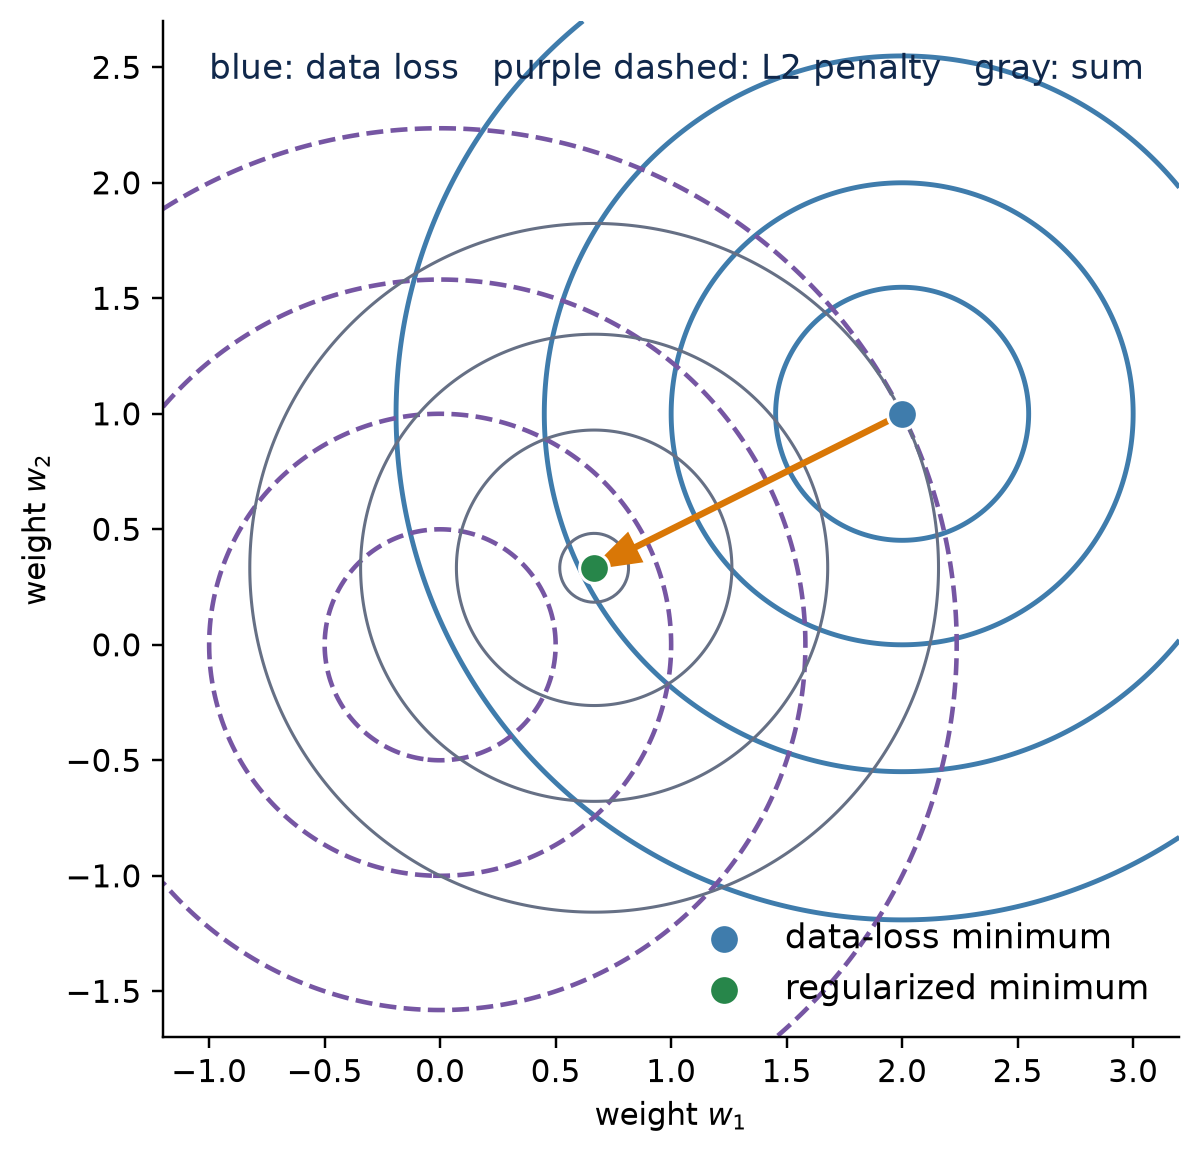
\includegraphics[width=0.88\linewidth,height=0.8\textheight,keepaspectratio]{l2-contours.png}
\end{frame}

\begin{frame}{L2 Is MAP Estimation under a Gaussian Prior}
  Assume independent weights and Gaussian observation noise:
  \[
    w_j\sim\mathcal N(0,\tau^2),
    \qquad
    y_i\mid\mathbf x_i,\mathbf w\sim
      \mathcal N(f_{\mathbf w}(\mathbf x_i),\sigma^2).
  \]
  Then
  \[
    -\log p(\mathbf w\mid D)
    =\frac1{2\sigma^2}\sum_i(y_i-f_{\mathbf w}(\mathbf x_i))^2
      +\frac1{2\tau^2}\|\mathbf w\|_2^2+\text{constant}.
  \]
  The zero mean expresses a prior preference for small weights, not knowledge that the true weights are zero.
\end{frame}

\begin{frame}{The Prior Scale Controls the Strength of the Belief}
  \centering
  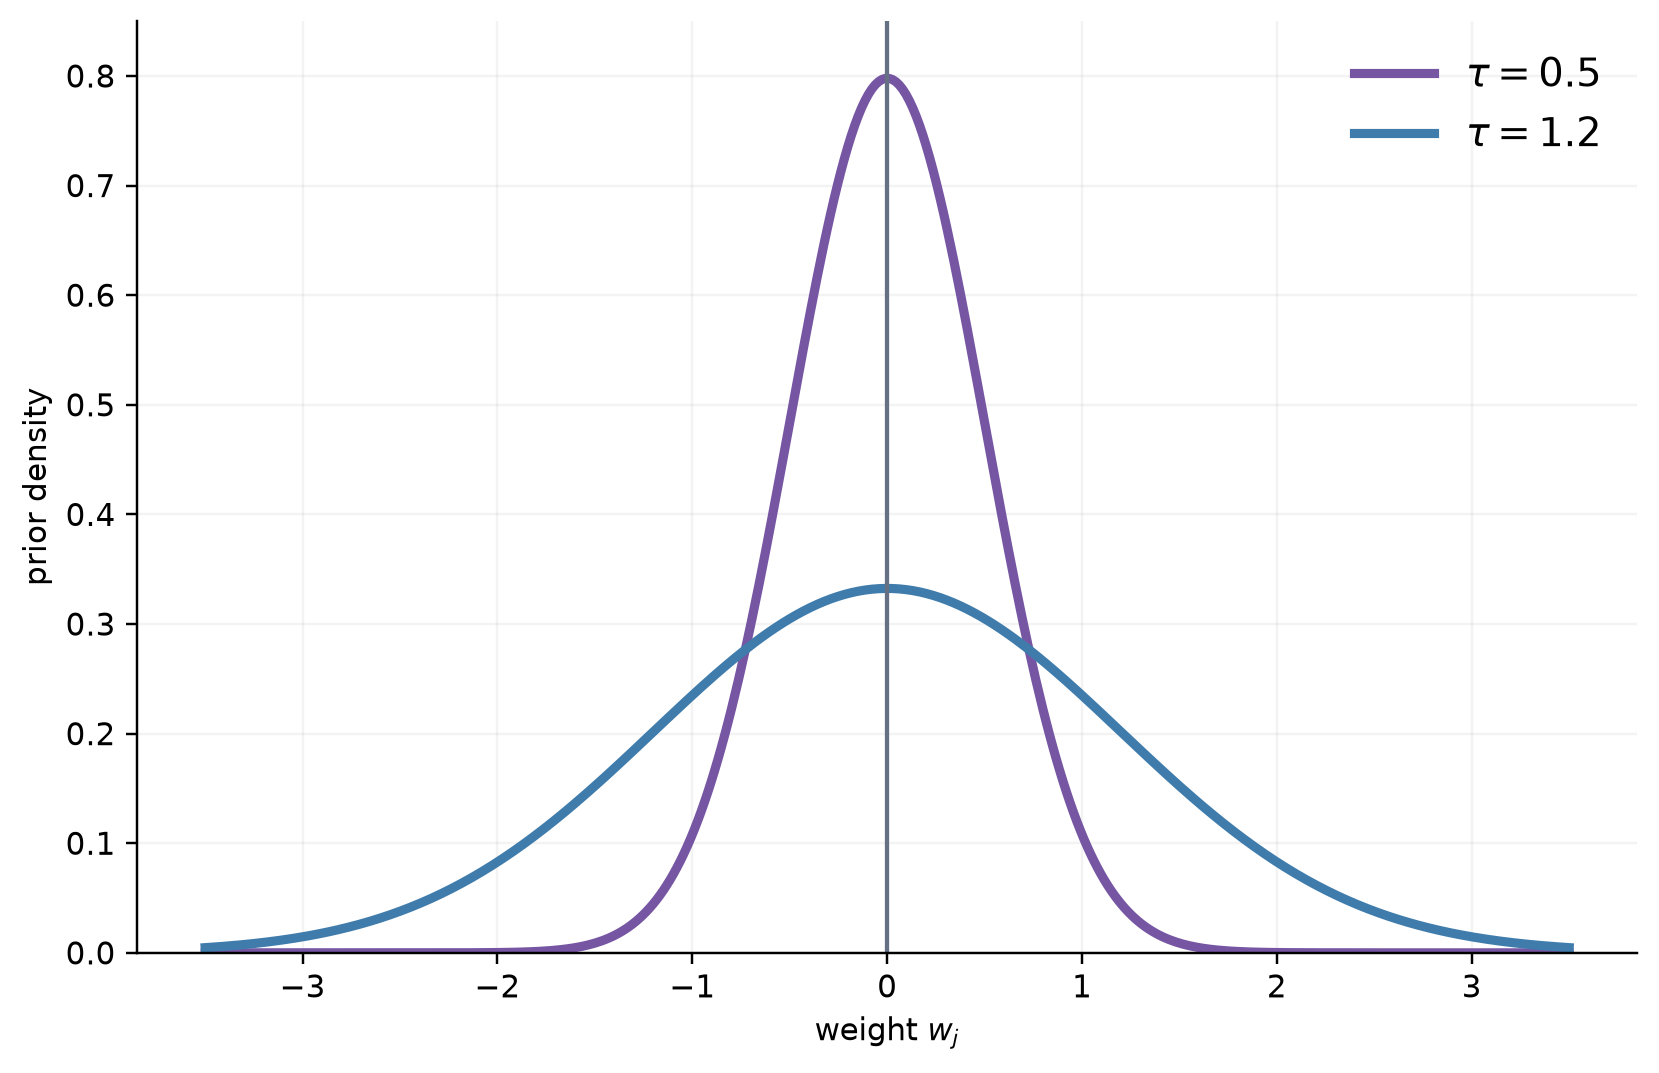
\includegraphics[width=0.94\linewidth,height=0.78\textheight,keepaspectratio]{weight-priors.png}
\end{frame}

\begin{frame}{L1 and L2 Impose Different Geometry}
  \centering
  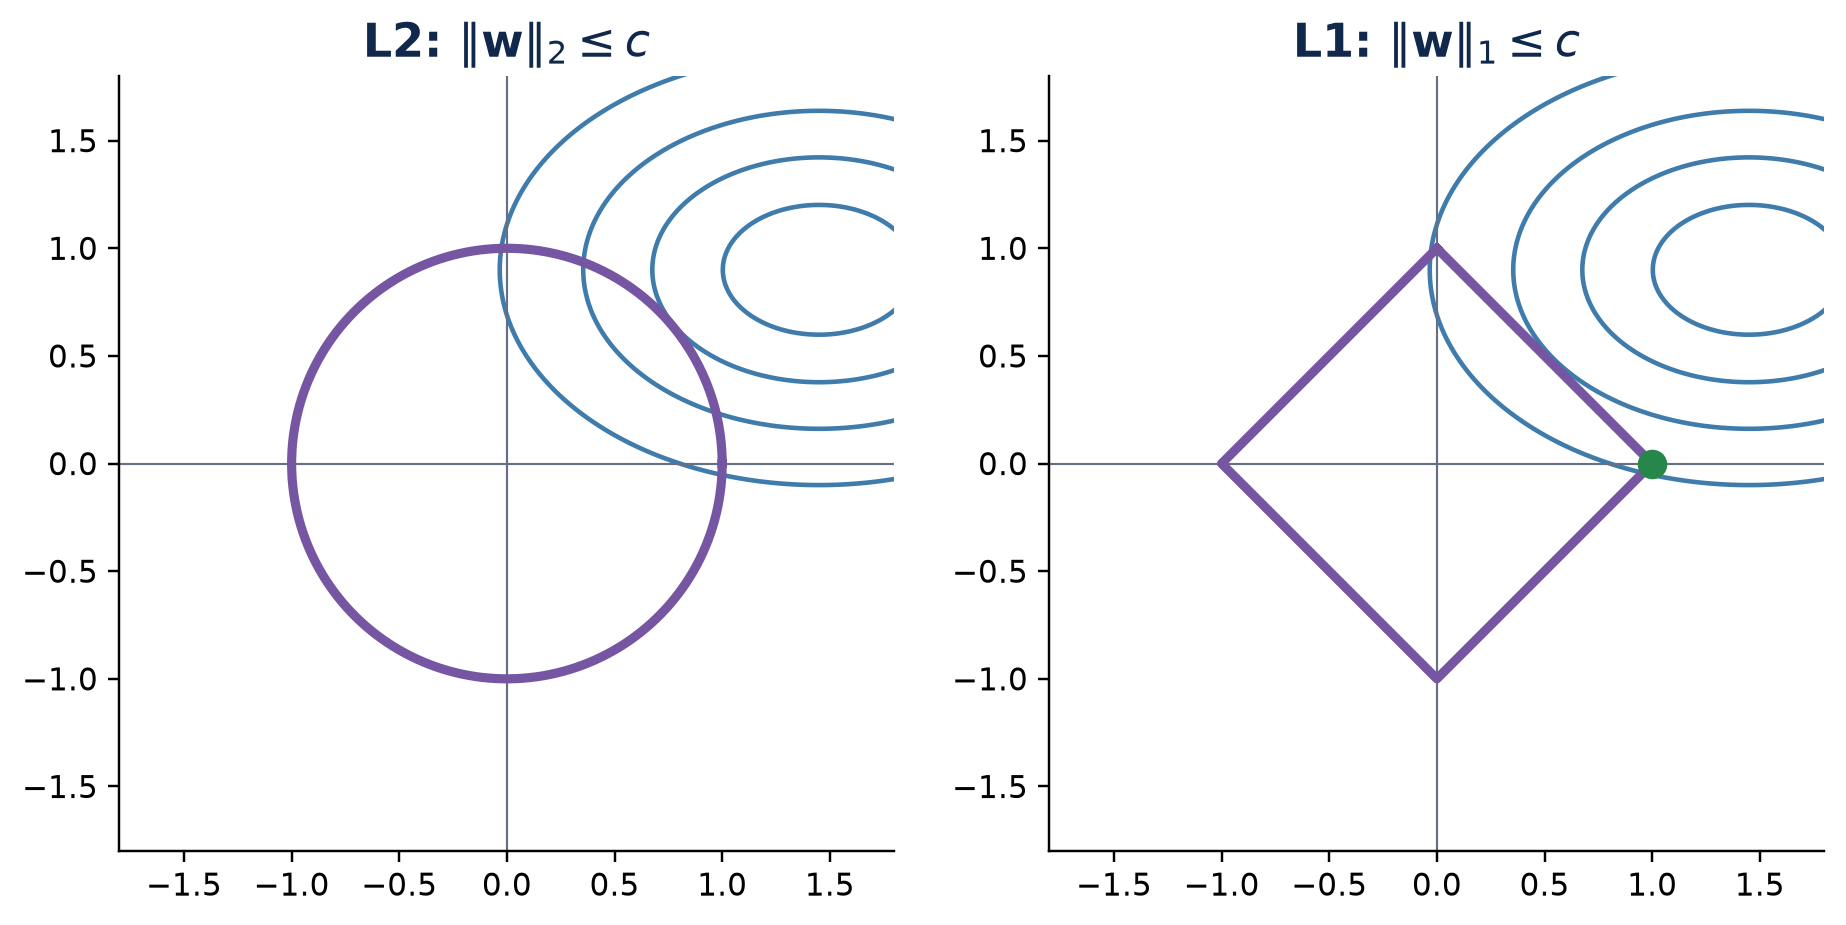
\includegraphics[width=0.98\linewidth,height=0.78\textheight,keepaspectratio]{l1-l2-geometry.png}
\end{frame}

\begin{frame}{L1 Corresponds to a Laplace Prior}
  \[
    p(w_j)=\frac1{2b}\exp\!\left(-\frac{|w_j|}{b}\right)
    \quad\Longrightarrow\quad
    -\log p(\mathbf w)=\frac1b\|\mathbf w\|_1+\text{constant}.
  \]
  The L1 ball has corners on coordinate axes. A loss contour can first touch at a corner,
  so exact zeros are common in convex linear models.
  Neural-network parameter symmetries make sparsity effects less direct.
\end{frame}

\begin{frame}{Increasing L2 Strength Shrinks Coefficients Continuously}
  \centering
  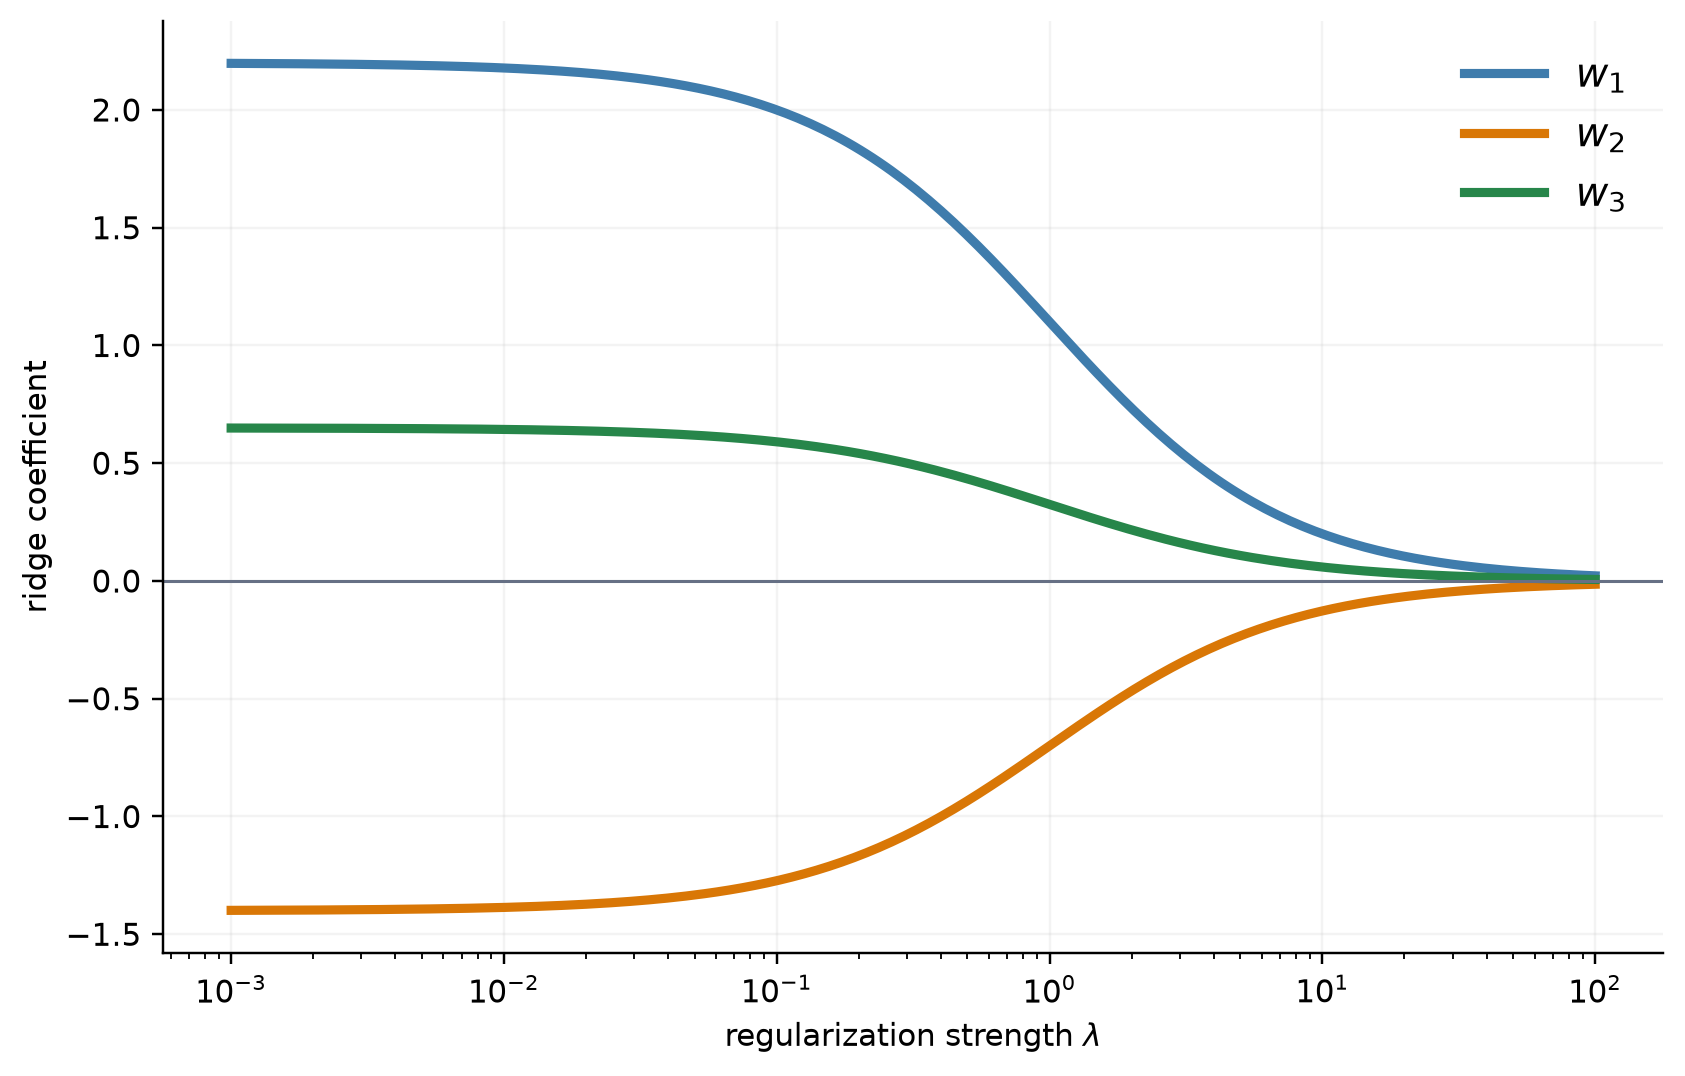
\includegraphics[width=0.95\linewidth,height=0.78\textheight,keepaspectratio]{regularization-path.png}
\end{frame}

\begin{frame}{Early Stopping Selects an Iterate}
  \centering
  \begin{tikzpicture}
    \begin{axis}[width=0.9\linewidth,height=0.68\textheight,xmin=0,xmax=10,ymin=0,ymax=1,
      xlabel={training epoch},ylabel={error},grid=both,legend style={draw=none,at={(0.98,0.98)},anchor=north east}]
      \addplot[courseblue,very thick,domain=0:10,samples=100] {0.75*exp(-0.35*x)+0.05};
      \addlegendentry{training}
      \addplot[courseorange,very thick,domain=0:10,samples=100] {0.55*exp(-0.5*x)+0.12+0.012*(x-4.7)^2};
      \addlegendentry{validation}
      \draw[coursegreen,very thick,dashed] (axis cs:5.45,0)--(axis cs:5.45,0.75);
      \node[coursegreen,font=\bfseries] at (axis cs:6.55,0.72) {restore best iterate};
    \end{axis}
  \end{tikzpicture}
\end{frame}

\begin{frame}{Averaging Can Reduce Estimator Variance}
  Let $M$ predictors have equal variance $v$ and pairwise error correlation $\rho$.
  Their average has variance
  \[
    \operatorname{Var}\!\left(\frac1M\sum_{m=1}^M\widehat f_m\right)
    =v\left(\rho+\frac{1-\rho}{M}\right).
  \]
  Averaging helps most when predictors are accurate enough and their errors are not perfectly correlated.
  It does not automatically remove shared bias.
\end{frame}

\begin{frame}{Bagging Creates Diversity by Resampling Data}
  \centering
  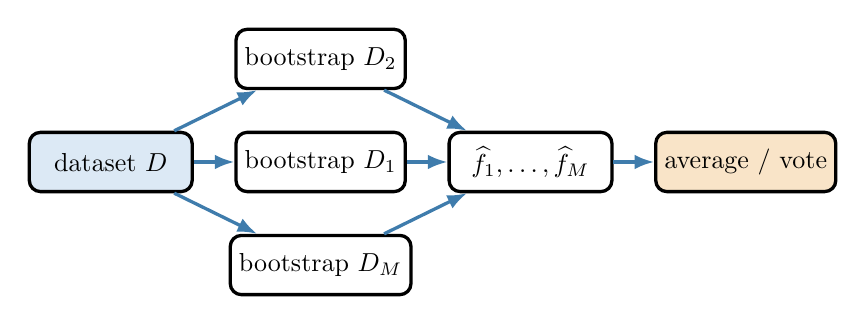
\begin{tikzpicture}[scale=0.94,transform shape,node distance=0.55cm,
    box/.style={draw,rounded corners,minimum width=2.2cm,minimum height=0.8cm,very thick,align=center},
    flow/.style={-{Latex[length=2.5mm]},very thick,courseblue}]
    \node[box,fill=courselightblue] (data) {dataset $D$};
    \node[box,right=of data] (b1) {bootstrap $D_1$};
    \node[box,above=of b1] (b2) {bootstrap $D_2$};
    \node[box,below=of b1] (bm) {bootstrap $D_M$};
    \node[box,right=of b1] (models) {$\widehat f_1,\ldots,\widehat f_M$};
    \node[box,fill=courselightorange,right=of models] (avg) {average / vote};
    \draw[flow] (data)--(b1); \draw[flow] (data)--(b2); \draw[flow] (data)--(bm);
    \draw[flow] (b1)--(models); \draw[flow] (b2)--(models); \draw[flow] (bm)--(models);
    \draw[flow] (models)--(avg);
  \end{tikzpicture}
\end{frame}

\begin{frame}{Dropout Samples a Smaller Network on Each Pass}
  \centering
  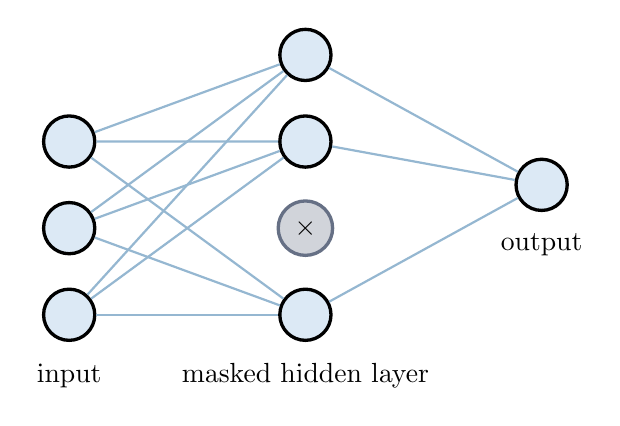
\begin{tikzpicture}[unit/.style={circle,draw,minimum size=0.65cm,very thick},
    kept/.style={unit,fill=courselightblue},dropped/.style={unit,fill=coursegray!30,draw=coursegray},
    edge/.style={courseblue!55,thick}]
    \foreach \y in {0,1,2}{\node[kept] (i\y) at (0,1.1*\y) {};}
    \node[kept] (h0) at (3,0) {}; \node[dropped] (h1) at (3,1.1) {$\times$};
    \node[kept] (h2) at (3,2.2) {}; \node[kept] (h3) at (3,3.3) {};
    \foreach \i in {0,1,2}{\foreach \h in {0,2,3}{\draw[edge] (i\i)--(h\h);}}
    \node[kept] (o) at (6,1.65) {};
    \foreach \h in {0,2,3}{\draw[edge] (h\h)--(o);}
    \node[below=0.15cm of i0] {input}; \node[below=0.15cm of h0] {masked hidden layer};
    \node[below=0.15cm of o] {output};
  \end{tikzpicture}

  A fresh Bernoulli mask is sampled during training; dropped units are not permanently deleted.
\end{frame}

\begin{frame}{Inverted Dropout Preserves the Expected Activation}
  For drop probability $p$,
  \[
    m_j\sim\operatorname{Bernoulli}(1-p),
    \qquad
    \widetilde{\mathbf h}
    =\frac{\mathbf m\odot\mathbf h}{1-p}.
  \]
  Conditioning on $\mathbf h$,
  \[
    \mathbb E_{\mathbf m}[\widetilde{\mathbf h}\mid\mathbf h]
    =\frac{\mathbb E[\mathbf m]\odot\mathbf h}{1-p}
    =\mathbf h.
  \]
  Dropout injects multiplicative noise and discourages fragile co-adaptation; it does not guarantee independent features.
\end{frame}

\begin{frame}{Standard Inference Uses the Full Network}
  \begin{center}
    \begin{tabular}{lll}
      \toprule
      & \textbf{Mask} & \textbf{Scale}\\
      \midrule
      Training & random Bernoulli & divide kept activations by $1-p$\\
      Inference & no units dropped & unchanged\\
      \bottomrule
    \end{tabular}
  \end{center}
  \vspace{0.5cm}
  Inverted dropout makes the deterministic inference scale match the training expectation.
  Monte Carlo dropout is a separate uncertainty method, not the default inference rule.
\end{frame}

\begin{frame}{Augmentation Averages Loss over Plausible Transformations}
  Let $T\sim q(T)$ transform an example while preserving its target. Train with
  \[
    L_{\mathrm{aug}}(\boldsymbol\theta)
    =\frac1n\sum_{i=1}^n
      \mathbb E_{T\sim q}
      [\ell(f_{\boldsymbol\theta}(T\mathbf x_i),y_i)].
  \]
  In practice, one or a few random transforms approximate this expectation per pass.
  The transformation distribution is a modeling assumption about which changes should not alter the target.
\end{frame}

\begin{frame}{One Cat, Several Label-Preserving Views}
  \centering
  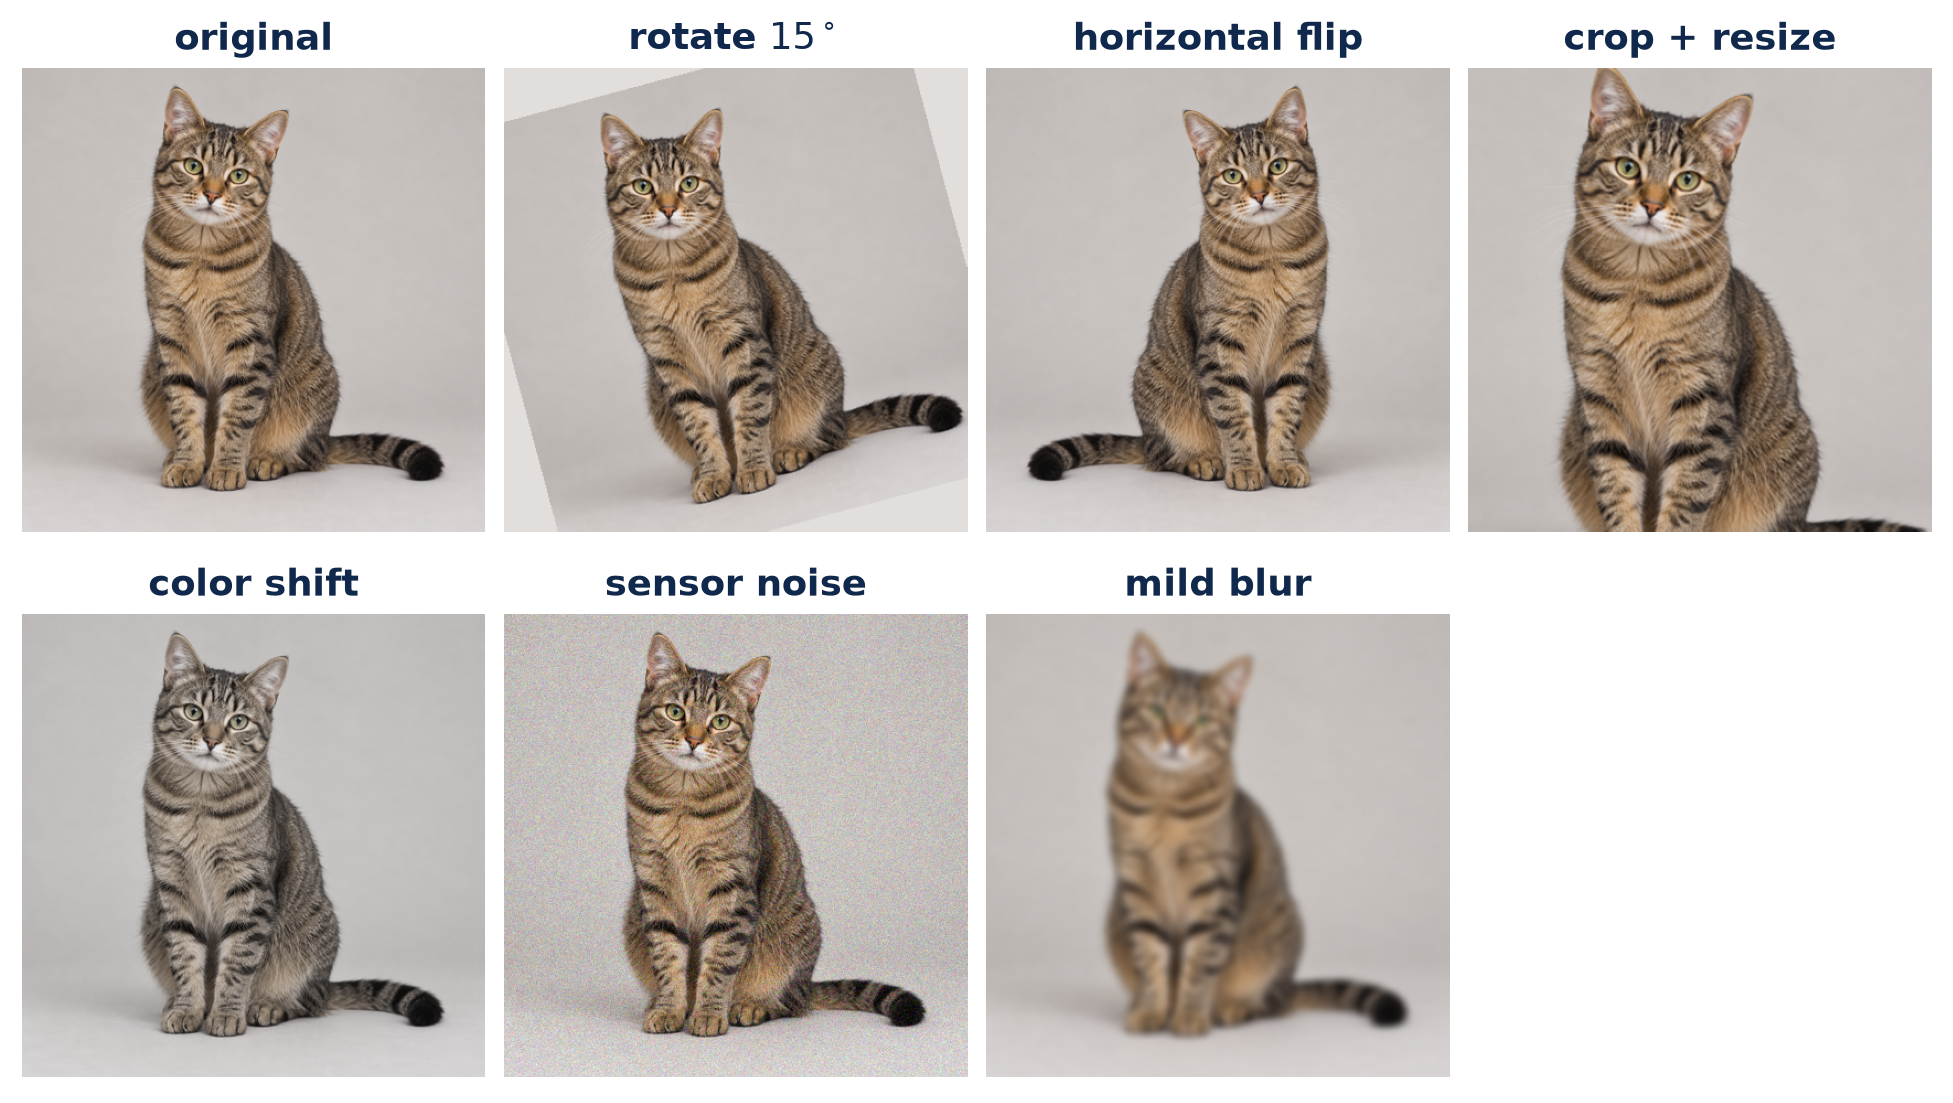
\includegraphics[width=0.98\linewidth,height=0.8\textheight,keepaspectratio]{augmentation-grid.png}
\end{frame}

\begin{frame}{Not Every Transformation Preserves the Target}
  \begin{itemize}
    \item Rotating a cat mildly usually preserves ``cat''; rotating a handwritten 6 may produce a 9.
    \item Horizontal reflection preserves many objects but reverses text, handedness, and chirality.
    \item Cropping is valid only while target-defining evidence remains visible.
    \item Noise and blur should resemble the sensor and deployment conditions.
  \end{itemize}
  Augmentation that changes the target creates systematic label noise.
\end{frame}

\begin{frame}{Augmentation and Equivariance Encode Related Beliefs}
  \begin{itemize}
    \item Augmentation teaches approximate behavior from transformed examples.
    \item An equivariant architecture enforces exact behavior within its mathematical assumptions.
    \item Invariance suits global labels; equivariance suits spatial or structured outputs.
  \end{itemize}
  The next lecture formalizes transformations, invariance, and equivariance before CNNs and GNNs.
\end{frame}

\begin{frame}{Choose the Control That Matches the Failure}
  \begin{itemize}
    \item High bias: improve representation, features, or optimization.
    \item High variance: add data, constrain the model, average predictors, or augment valid symmetries.
    \item L1/L2 express parameter preferences; early stopping constrains training time.
    \item Dropout and augmentation inject structured training noise.
  \end{itemize}
  Select every strength or stopping rule on validation data. Use the test set once for the final estimate.
\end{frame}

\end{document}
